% Eval-first ordering + measurement-with-uncertainty for Ch23 ("Evaluating an Agent").
% Standalone TikZ; compiled by `book-scaffold build-figures` via pdflatex -> pdftocairo -> SVG.
% Top row, left-to-right: define the eval TARGET first -> harness built TOWARD it (a back-arrow
% makes "toward, not the reverse" visible) -> a small failure-derived task suite -> each run
% resampled over multiple epochs -> result reported as a value WITH an error bar (not a bare point).
% The "a score without an error bar is not a result" idea is the caption strip beneath.
\documentclass[tikz,border=4mm]{standalone}
\usepackage{tikz}
\usetikzlibrary{positioning, arrows.meta, calc}

\begin{document}
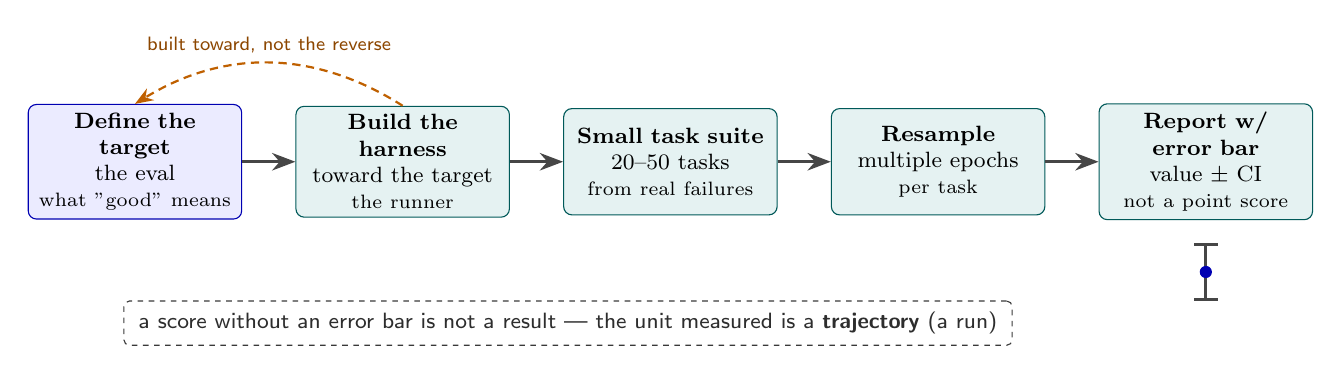
\begin{tikzpicture}[
  font=\sffamily,
  target/.style={draw=blue!70!black, fill=blue!8, rounded corners=3pt, align=center,
    text width=2.5cm, minimum height=1.35cm, inner sep=3pt, font=\footnotesize},
  stage/.style={draw=teal!70!black, fill=teal!10, rounded corners=3pt, align=center,
    text width=2.5cm, minimum height=1.35cm, inner sep=3pt, font=\footnotesize},
  flow/.style={-Stealth, very thick, draw=gray!55!black},
  back/.style={-Stealth, thick, draw=orange!75!black, dash pattern=on 3pt off 2pt}
]

% the eval TARGET first (highlighted), then the four stages built toward it
\node[target] (s1) at (0,0)    {\textbf{Define the target}\\the eval\\{\scriptsize what "good" means}};
\node[stage]  (s2) at (3.4,0)  {\textbf{Build the harness}\\toward the target\\{\scriptsize the runner}};
\node[stage]  (s3) at (6.8,0)  {\textbf{Small task suite}\\20--50 tasks\\{\scriptsize from real failures}};
\node[stage]  (s4) at (10.2,0) {\textbf{Resample}\\multiple epochs\\{\scriptsize per task}};
\node[stage]  (s5) at (13.6,0) {\textbf{Report w/ error bar}\\value $\pm$ CI\\{\scriptsize not a point score}};

\draw[flow] (s1) -- (s2);
\draw[flow] (s2) -- (s3);
\draw[flow] (s3) -- (s4);
\draw[flow] (s4) -- (s5);

% back-arrow: the harness is built TOWARD the target, not the reverse
\draw[back] (s2.north) to[bend right=32] node[midway, above, font=\sffamily\scriptsize, text=orange!55!black] {built toward, not the reverse} (s1.north);

% a tiny value-with-error-bar glyph under the last stage, to make "with an error bar" literal
\draw[very thick, gray!55!black] (13.6,-1.05) -- (13.6,-1.75);
\draw[very thick, gray!55!black] (13.45,-1.05) -- (13.75,-1.05);
\draw[very thick, gray!55!black] (13.45,-1.75) -- (13.75,-1.75);
\fill[blue!70!black] (13.6,-1.4) circle (2.2pt);

% caption strip beneath
\node[draw=gray!45!black, dash pattern=on 2pt off 2pt, rounded corners=2pt, align=center,
  text width=11.0cm, inner sep=4pt, font=\sffamily\footnotesize, text=gray!35!black]
  at (5.5,-2.05) {a score without an error bar is not a result --- the unit measured is a \textbf{trajectory} (a run)};

\end{tikzpicture}
\end{document}
